\section{Experimental Protocol}\label{sec:experiments}
The protocol asks four distinct questions. Q1 measures predictive accuracy and macro-F1 under matched topology and training. Q2 measures fidelity to held-out real features, including minority-sensitive metrics. Q3 varies packet budgets and component controls to expose the representation--communication frontier. Q4 compares local extraction with a shared encoder snapshot to determine whether apparent modes survive a coordinate-compatibility control.

The implementation supports CIFAR-100 classification in the prepared MiSFP matrix; inherited H-SFP also contains CIFAR-10, HAM10000, ImageNet, and segmentation paths, but those are not claimed as validated MiSFP targets. All reported runs use 200 clients attached to five edges, a client fraction of $0.1$ per round, 60 communication rounds, Adam with learning rate $10^{-4}$ and local batch size 16, inherited synchronization intervals $t_1=5$ and $t_2=10$, and a ResNet-18 split after the client layer-2/GAP output ($d_{ce}=128$) with an edge projection to $d_{ec}=256$; the settings are taken from the resolved configuration recorded with every run (\cref{tab:setup}). Seeds are predefined as $\{1,2,3\}$ in the result manifest, and all 31 registered configurations completed for all three seeds (93 runs). Reported uncertainty is sample standard deviation across completed seeds; for one seed it is unavailable, never zero.

\begin{table*}[t]\caption{Datasets, partitions, and evaluation configuration. ``Planned'' fields are protocol choices, not completed runs.}\label{tab:setup}\centering\small
\resizebox{\textwidth}{!}{\begin{tabular}{llllllllll}\toprule
Dataset & Task/classes & Split & Clients/edges & Participation & Heterogeneity & Model/split & Metrics & Seeds & Status\\\midrule
CIFAR-100 & class./100 & standard train/test; train-val 0.1 & 200/10 & resolved config & IID, Dirichlet $\alpha$ sweep & ResNet-18; 128/256 dims & Acc., macro-F1, fidelity, bytes & 1,2,3 & supported/planned\\
CIFAR-10 & class./10 & inherited & unresolved & unresolved & IID/non-IID & inherited & Acc., macro-F1 & 1,2,3 & inherited, not yet integrated\\
HAM10000 & class./7 & inherited patient-aware split to verify & unresolved & unresolved & non-IID & ResNet-50/VGG & balanced metrics & 1,2,3 & planned adaptation\\
\bottomrule\end{tabular}}\end{table*}

\begin{table*}[t]\caption{Main predictive performance. Entries will be mean $\pm$ sample SD across seeds 1--3; \MissingResult{} denotes unmeasured, not zero.}\label{tab:main}\centering\small
\resizebox{\textwidth}{!}{\begin{tabular}{llcccccc}\toprule
Dataset & Partition & FedAvg$^\dagger$ & SplitFed$^\dagger$ & FedProto$^\dagger$ & H-SFP & MiSFP-K1 & MiSFP-Adaptive\\\midrule
CIFAR-100 & IID, accuracy (\%) & \MissingResult&\MissingResult&\MissingResult&\MissingResult&\MissingResult&\MissingResult\\
 & IID, macro-F1 (\%) & \MissingResult&\MissingResult&\MissingResult&\MissingResult&\MissingResult&\MissingResult\\
 & Dirichlet $\alpha$ (resolved), accuracy (\%) & \MissingResult&\MissingResult&\MissingResult&\MissingResult&\MissingResult&\MissingResult\\
 & Dirichlet $\alpha$ (resolved), macro-F1 (\%) & \MissingResult&\MissingResult&\MissingResult&\MissingResult&\MissingResult&\MissingResult\\
\bottomrule\multicolumn{8}{l}{\footnotesize $^\dagger$Adapted/contextual until rerun under the same hierarchy and budget. No winners are predesignated.}
\end{tabular}}\end{table*}

\begin{table*}[t]\caption{Communication and resource cost. CIFAR-100, Dir($\alpha{=}0.1$), 60 rounds; mean $\pm$ sample SD over seeds. Formulas are analytical; total communication is the runtime tracker total (MB) including model synchronization; $^\ast$H-SFP does not use the serialized MiSFP packet format. Unmeasured fields remain \MissingResult. Runtime and peak memory were measured with up to twelve concurrent runs sharing one RTX 6000 Ada GPU; they indicate cost but are not controlled timing comparisons.}\label{tab:resources}\centering\small
\resizebox{\textwidth}{!}{\begin{tabular}{lccccccc}\toprule
Method & C--E payload (MiB) & E--C payload (MiB) & Model sync. (MiB) & Total (MiB) & Runtime (s) & Peak memory (MiB) & Analytical packet body\\\midrule
\tabrows{generated/misfp_resources_rows.tex}
\bottomrule\end{tabular}}\end{table*}

\begin{table}[t]\caption{Component ablations on CIFAR-100, Dir($\alpha{=}0.1$); final-round metrics, mean $\pm$ SD across seeds; components/class is the edge-to-cloud output in the final round.}\label{tab:ablation}\centering\small
\resizebox{\columnwidth}{!}{\begin{tabular}{lccc}\toprule Variant & Accuracy (\%) & Macro-F1 (\%) & Components/class\\\midrule
\tabrows{generated/misfp_ablation_rows.tex}
\bottomrule\end{tabular}}\end{table}

\begin{table*}[t]\caption{Budget and complexity sensitivity. CIFAR-100, Dir($\alpha{=}0.1$). Every row corresponds to a resolved configuration and seed set; payload column reports total communication (MB). Runtime and peak memory were measured with up to twelve concurrent runs sharing one RTX 6000 Ada GPU; they indicate cost but are not controlled timing comparisons.}\label{tab:sensitivity}\centering\small
\resizebox{\textwidth}{!}{\begin{tabular}{lcccccccc}\toprule
Budget rule & Precision & Cap & Min. support & Boundary samples & Accuracy (\%) & Macro-F1 (\%) & Payload (MiB) & Runtime (s)\\\midrule
\tabrows{generated/misfp_sensitivity_rows.tex}
\bottomrule\end{tabular}}\end{table*}

\begin{table*}[t]\caption{Representation fidelity and alignment diagnostic on held-out real features. Lower is better for NLL/SWD/MMD; higher is better for coverage/recall.}\label{tab:fidelity}\centering\small
\resizebox{\textwidth}{!}{\begin{tabular}{llcccccc}\toprule
Extraction & Representation & NLL (nat/dim) & SWD & MMD & Mode coverage (\%) & Minority recall (\%) & Between-source ratio\\\midrule
Local & single Gaussian & \MissingResult&\MissingResult&\MissingResult&\MissingResult&\MissingResult&\MissingResult\\
Local & MiSFP mixture & \MissingResult&\MissingResult&\MissingResult&\MissingResult&\MissingResult&\MissingResult\\
Shared snapshot & single Gaussian & \MissingResult&\MissingResult&\MissingResult&\MissingResult&\MissingResult&\MissingResult\\
Shared snapshot & MiSFP mixture & \MissingResult&\MissingResult&\MissingResult&\MissingResult&\MissingResult&\MissingResult\\
\bottomrule\end{tabular}}\end{table*}


\paragraph{Baselines and comparability.}
H-SFP is the direct inherited baseline. MiSFP-K1 isolates the new support-weighted packet/pooling path; MiSFP-Edge isolates across-client retention; fixed $K$ and adaptive variants add within-client components. FedAvg, SplitFed, and FedProto are contextual or adapted baselines unless run with matched partitions, model capacity, optimization budget, and hierarchy. Published values are not mixed with reruns.

\paragraph{Metrics.}
Predictive metrics are top-1 accuracy and macro-F1. Communication reports exact serialized prototype bytes at each boundary and total bytes including model synchronization. Fidelity is evaluated on held-out real features extracted by the stated encoder mode using per-class NLL, sliced Wasserstein distance (SWD; lower is better), maximum mean discrepancy (MMD; lower is better), nearest-mode coverage (higher is better), and minority-component recall after a preregistered clustering/projection fit on training features only. Resource measurements report wall-clock seconds and peak allocated memory with hardware/software metadata.

The tables were designed to test alternatives rather than presuppose gains. Better fidelity without predictive change would indicate that the classifier is insensitive to retained modes; higher cost without fidelity improvement would argue against extra components; degradation under local but not shared-snapshot extraction would implicate coordinate mismatch; and matched-byte improvement would support allocation rather than payload size as the operative factor.

\subsection{Results}\label{sec:results}
All values below are final-round (round 60) test metrics, reported as mean $\pm$ sample SD over seeds 1--3; every configuration has $n=3$. With three seeds we describe differences relative to the seed-to-seed SD and make no significance claims.

\paragraph{Predictive quality (Q1).}
Under Dir($\alpha{=}0.1$) (\cref{tab:ablation}), H-SFP reaches $12.66\pm0.36\%$ accuracy and MiSFP-K1 $12.29\pm0.11\%$, so the new support-weighted packet path alone does not change accuracy. Retaining source components at the edge (MiSFP-Edge) gives $13.99\pm0.06\%$, and fixed local mixtures give $15.92\pm0.16\%$ (K2) and $16.63\pm0.31\%$ (K4); the K4--H-SFP gap of $3.97$ percentage points is more than ten times the larger seed SD, and macro-F1 follows the same order ($11.62\pm0.29\%$ for H-SFP, $15.05\pm0.45\%$ for K4). The same ordering of H-SFP/K1 below the retaining variants holds under IID and Dir($\alpha{=}0.7$) (\cref{tab:main}): across-client retention adds $4.94$ (IID), $4.10$ (Dir $0.7$), and $1.70$ (Dir $0.1$) points over MiSFP-K1, matching the number of edge-to-cloud components it retains ($3.35$, $2.84$, and $1.58$ per class, respectively). Fixed local mixtures add little beyond retention under IID (K2 $15.50\pm0.35\%$ versus Edge $15.32\pm0.23\%$) but add $1.93$ points under Dir($\alpha{=}0.1$). Absolute accuracy remains low for every method in this 60-round configuration, so the results characterize relative behavior within this protocol rather than competitive CIFAR-100 accuracy.

\paragraph{Adaptive selection.}
MiSFP-Adaptive ($14.67\pm0.14\%$ under Dir $0.1$) lies between MiSFP-Edge and the fixed mixtures and retains $1.66$ components per class against $1.58$ for Edge, so the held-out-likelihood rule rarely accepts a second local component. Under IID its three runs coincide with MiSFP-Edge in accuracy, components, and bytes for every seed, consistent with the rule selecting one local component throughout. Lowering the minimum support from 10 to 1 raises its accuracy from $14.40\pm0.26\%$ to $14.91\pm0.09\%$, and the boundary sample count (10, 50, 200 per component) changes accuracy by at most $0.22$ points (\cref{tab:sensitivity,fig:diagnostics}).

\paragraph{Communication and budgets (Q3).}
Total communication over 60 rounds is dominated by model synchronization: $1362.4$\,MB for H-SFP, $1417.4$\,MB for K2, and $1433.0$\,MB for K4, so the extra components cost $4.0\%$ and $5.2\%$ more in total (\cref{tab:resources}). A float16 K2 packet matched to the MiSFP-K1 byte budget uses $1348.4$\,MB in total, less than MiSFP-K1 ($1364.2$\,MB), and still reaches $16.03\pm0.31\%$; enlarging the K2 budget to $1.5\times$ or $2.0\times$ does not improve on this ($15.65\pm0.24\%$, $16.04\pm0.07\%$). For this setting the gain is therefore attributable to how the budget is allocated across components rather than to payload size. The adaptive variant is insensitive to the budget ($14.49$--$14.66\%$).

\paragraph{Fidelity and alignment (Q2, Q4).}
On held-out features (\cref{tab:fidelity}), MiSFP-K2 mixtures have lower SWD and MMD than their moment-collapsed single Gaussian under both extraction modes (local SWD $0.051$ versus $0.053$, MMD $0.122$ versus $0.137$), but a higher (worse) per-dimension NLL ($-0.312\pm0.339$ versus $-0.867\pm0.037$) with large seed variation, so the fidelity evidence is mixed and the sample-based distances improve only modestly. Extracting with a shared encoder snapshot lowers the between-source dispersion ratio from $0.474\pm0.049$ to $0.346\pm0.078$ and raises MiSFP-K2 accuracy from $15.92\pm0.16\%$ to $17.43\pm0.05\%$, while MiSFP-K1 is unchanged ($12.21\pm0.47\%$ versus $12.29\pm0.11\%$). Part of the source dispersion retained under local extraction thus reflects encoder-coordinate mismatch, and mixtures benefit more from compatible coordinates than single components do. The snapshot control is not a free improvement: broadcasting the snapshot raises total communication to about $4.5$\,GB per run, roughly $3.2\times$ the local-extraction total.

\begin{figure*}[t]
\centering\IfFileExists{figures/empirical_results.pdf}{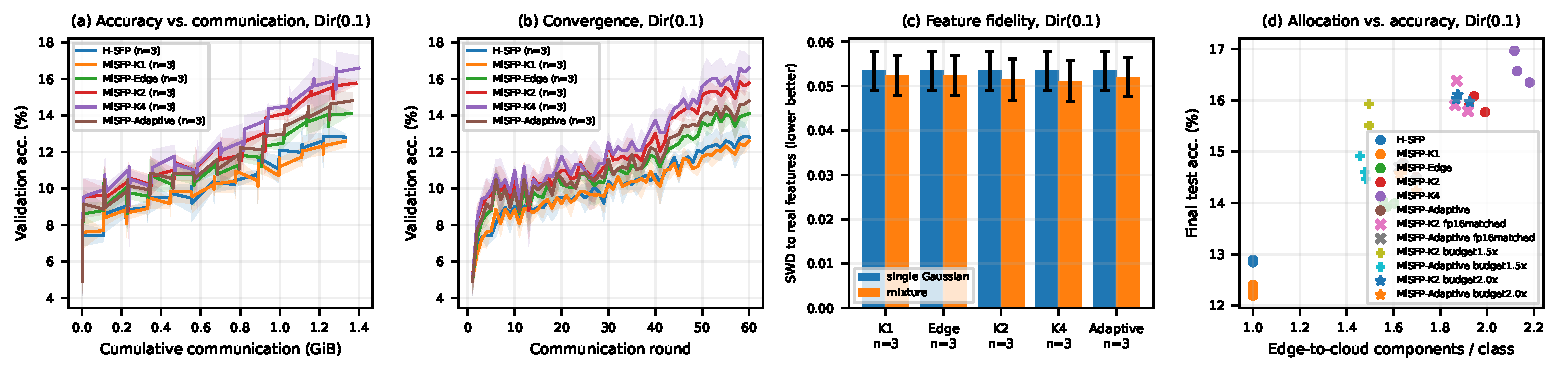
\includegraphics[width=.98\textwidth]{figures/empirical_results.pdf}}{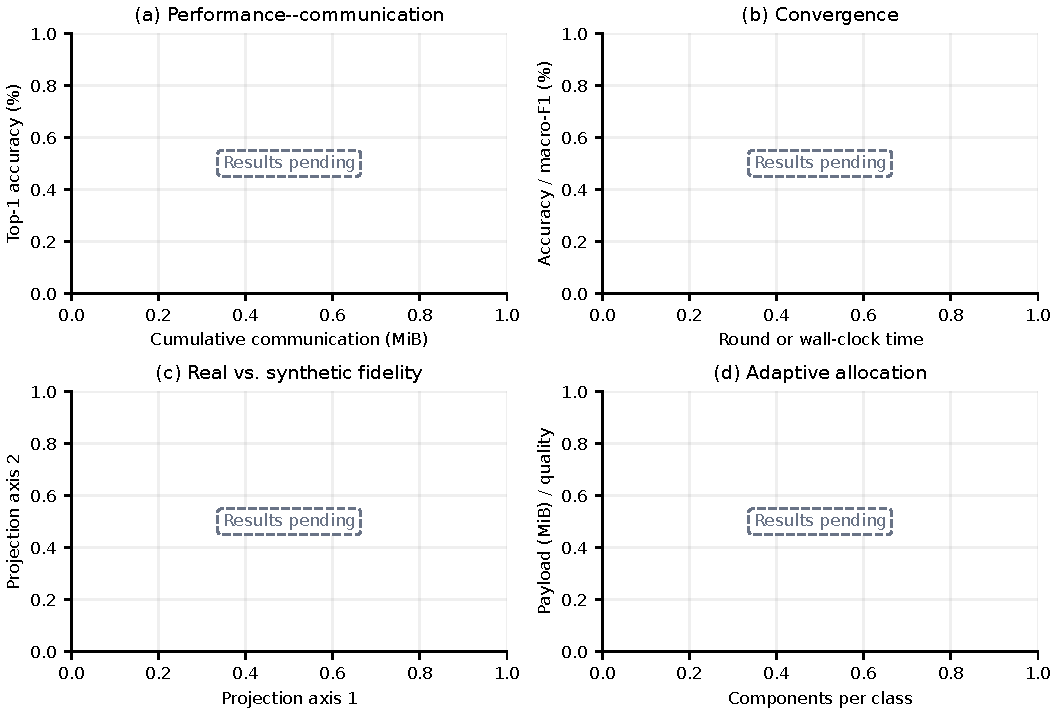
\includegraphics[width=.98\textwidth]{figures/empirical_templates.pdf}}
\caption{Empirical results generated from the central long-format result file (validated runs only; CIFAR-100, Dir($\alpha{=}0.1$)). (a) Validation accuracy versus cumulative communication; (b) validation accuracy versus communication round; (c) sliced Wasserstein distance between synthetic and real training features in a PCA projection fit on real features, single Gaussian versus mixture; (d) edge-to-cloud components per class versus final-round test accuracy, including the matched-budget variants. Lines and bars show seed means; bands and error bars are $\pm1$ sample SD when at least two seeds are complete; $n$ gives the completed seeds per series. Panels without a completed run are marked results pending.}
\label{fig:empirical}
\end{figure*}

\begin{figure*}[t]
\centering\IfFileExists{figures/diagnostic_results.pdf}{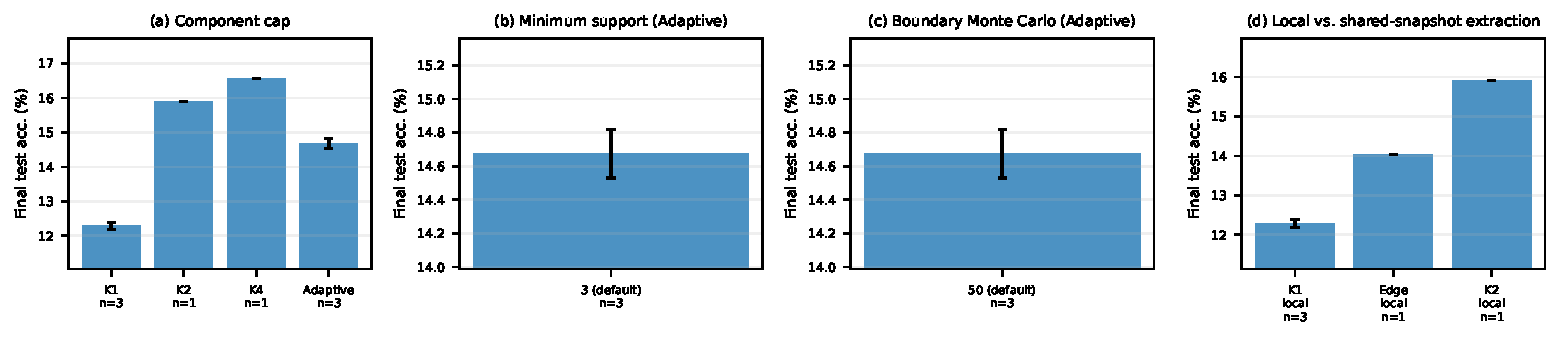
\includegraphics[width=.98\textwidth]{figures/diagnostic_results.pdf}}{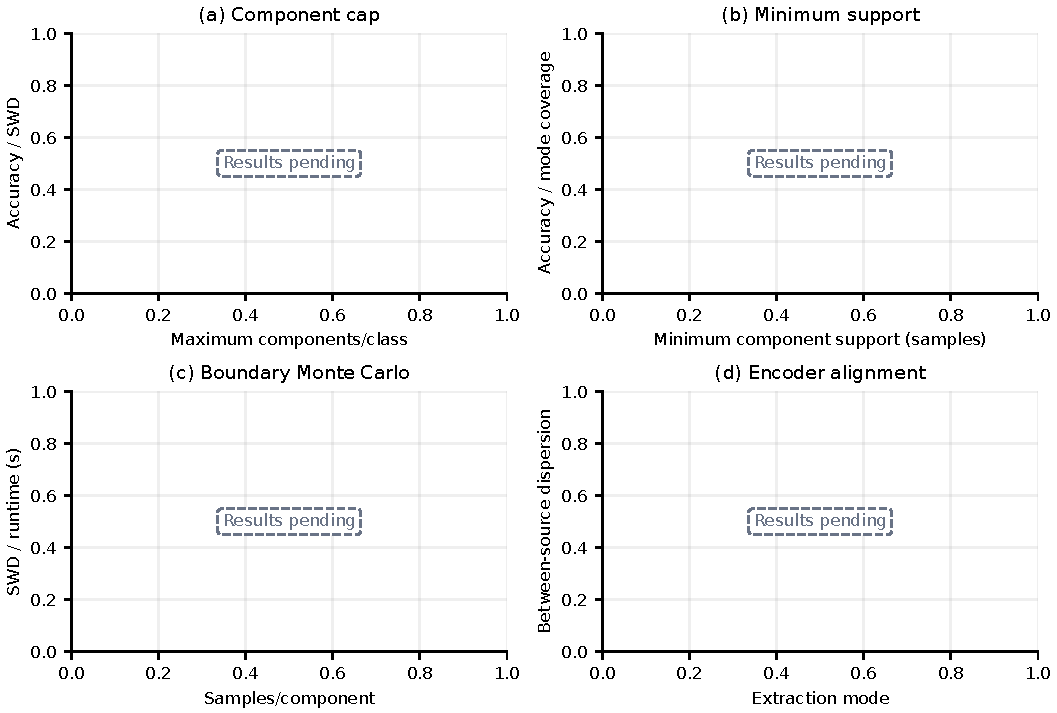
\includegraphics[width=.98\textwidth]{figures/diagnostic_templates.pdf}}
\caption{Sensitivity and alignment diagnostics on CIFAR-100, Dir($\alpha{=}0.1$): final-round test accuracy for (a) component cap (K1, K2, K4, adaptive), (b) minimum support (adaptive), (c) boundary Monte Carlo samples per component (adaptive), and (d) local versus shared-snapshot extraction. Bars are seed means with $\pm1$ sample SD when at least two seeds are complete; $n$ is shown under each bar; panels without a completed run are marked results pending.}
\label{fig:diagnostics}
\end{figure*}
